% AI-assisted code: generated and revised with Claude Opus 5.5
% under the author's direction; reviewed and tested by the author
% (see the thesis section "Use of AI tools").
% UML state machine of a candidate (candidate.py: CandidateState, _TRANSITIONS).
\documentclass[border=4pt]{standalone}
% Shared TikZ style for the thesis UML figures (standalone documents).
\usepackage[T1]{fontenc}
\usepackage{lmodern}
\usepackage{tikz}
\usetikzlibrary{positioning,arrows.meta,shapes.multipart,shapes.geometric,fit,backgrounds,calc,matrix}
\definecolor{umlfill}{HTML}{F4F6FA}
\definecolor{umlline}{HTML}{3A4150}
\definecolor{umlaccent}{HTML}{0071E3}
\tikzset{
  every node/.style={font=\sffamily\small},
  % class box: \node[class] {Name \nodepart{second} attrs \nodepart{third} ops};
  class/.style={rectangle split, rectangle split parts=3, draw=umlline, fill=umlfill,
    align=left, rectangle split part align={center,left,left}, inner sep=3pt, font=\sffamily\scriptsize},
  % generalisation (hollow triangle), realisation (dashed, hollow triangle)
  inherit/.style={-{Triangle[open,length=7pt,width=7pt]}, draw=umlline},
  realize/.style={-{Triangle[open,length=7pt,width=7pt]}, dashed, draw=umlline},
  % composition (filled diamond at the whole), aggregation (hollow), association, dependency
  compose/.style={{Diamond[length=9pt,width=6pt]}-, draw=umlline},
  aggregate/.style={{Diamond[open,length=9pt,width=6pt]}-, draw=umlline},
  assoc/.style={-, draw=umlline},
  navassoc/.style={-{Straight Barb[length=5pt]}, draw=umlline},
  depend/.style={-{Straight Barb[length=5pt]}, dashed, draw=umlline},
  mult/.style={font=\sffamily\tiny, inner sep=1pt},
  stereo/.style={font=\sffamily\tiny\itshape},
}

\begin{document}
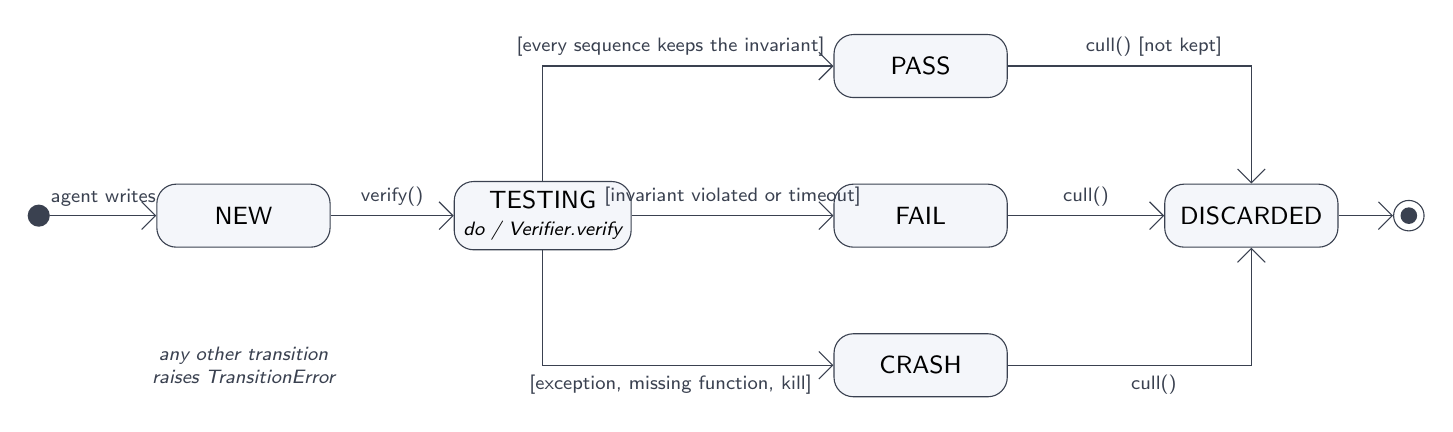
\begin{tikzpicture}[
    state/.style={rectangle, rounded corners=7pt, draw=umlline, fill=umlfill, minimum width=22mm,
                  minimum height=8mm, align=center},
    tr/.style={-{Straight Barb[length=5pt]}, draw=umlline},
    lbl/.style={font=\sffamily\scriptsize, align=center, text=umlline}]
  \node[circle, fill=umlline, minimum size=8pt, inner sep=0] (init) at (0,0) {};
  \node[state] (new) at (2.6,0) {NEW};
  \node[state] (testing) at (6.4,0) {TESTING\\[-1pt]{\scriptsize\itshape do / Verifier.verify}};
  \node[state] (pass) at (11.2,1.9) {PASS};
  \node[state] (fail) at (11.2,0) {FAIL};
  \node[state] (crash) at (11.2,-1.9) {CRASH};
  \node[state] (disc) at (15.4,0) {DISCARDED};
  \node[circle, draw=umlline, minimum size=11pt, inner sep=0] (fin) at (17.4,0) {};
  \node[circle, fill=umlline, minimum size=6pt, inner sep=0] at (fin) {};

  \draw[tr] (init) -- node[lbl, above] {agent writes} (new);
  \draw[tr] (new) -- node[lbl, above] {verify()} (testing);
  \draw[tr] (testing.north) |- node[lbl, above, pos=0.72] {[every sequence keeps the invariant]} (pass.west);
  \draw[tr] (testing.east) -- node[lbl, above] {[invariant violated or timeout]} (fail.west);
  \draw[tr] (testing.south) |- node[lbl, below, pos=0.72] {[exception, missing function, kill]} (crash.west);
  \draw[tr] (pass.east) -| node[lbl, above, pos=0.3] {cull() [not kept]} (disc.north);
  \draw[tr] (fail.east) -- node[lbl, above] {cull()} (disc.west);
  \draw[tr] (crash.east) -| node[lbl, below, pos=0.3] {cull()} (disc.south);
  \draw[tr] (disc) -- (fin);
  \node[lbl, font=\sffamily\scriptsize\itshape] at (2.6,-1.9)
    {any other transition\\raises TransitionError};
\end{tikzpicture}
\end{document}
